\documentclass[12pt,a4paper]{article}
\usepackage[utf8]{inputenc}
\usepackage[utf8]{vietnam} %Bien dich duoc tieng Viet
\usepackage{amsmath,amsfonts,amssymb} %Font toan
\usepackage{type1cm}
\usepackage{graphicx}
\usepackage{subfig}
\graphicspath{ {images/} }
\usepackage{multirow}
\usepackage{multicol}
\usepackage{comment}
\usepackage[unicode]{hyperref} %Tu dong tao bookmark
\usepackage{indentfirst} %Thut vao dau dong o tat ca cac doan
\usepackage{color} %Mau sac
\usepackage[left=2cm,right=2cm,top=2cm,bottom=2cm]{geometry}
\usepackage[american,cuteinductors,smartlabels]{circuitikz}
\usepackage{sagetex}
\usepackage{tikz}
\usetikzlibrary{arrows, decorations.markings, calc, fadings, decorations.pathreplacing, patterns, decorations.pathmorphing, positioning}	
\title{\textbf{Bài tập ngắn mạch}}
\author{SVTH: Thi Minh Nhựt -- Email: thiminhnhut@gmail.com}
\date{Ngày 28 tháng 08 năm 2016}
\newcommand{\viss}[1]{#1_\text{\textit{đm}}} % Subscript tiếng Việt trong công thức toán
\newcommand{\vidss}[2]{#1_\text{\textit{đm#2}}}
\newcommand{\vids}[3]{#1_{#2\text{\textit{đm#3}}}}
\newcommand{\unit}[1]{~#1}							% Sau số có cách khoảng đơn vị
\newcommand{\unitp}[1]{~\left({#1}\right)} %Cặp dấu ngoặc của đơn vị
\newcommand{\pfm}[1]{\left({#1}\right)} %Cặp dấu ngoặc trong công thức
\newcommand{\bigf}[1]{\small{#1}} % Ký hiệu cho máy phát
\newcommand{\bbigf}[1]{\huge{#1}} % Tên của các phần tử
\newcommand{\drawe}{\draw[line width=1.2pt]}

\begin{document}
\maketitle
\everymath{\displaystyle}
\pagenumbering{arabic}
\subsubsection*{Bài tập 1}
\subparagraph{Đề bài} Cho sơ đồ nguyên lý của nhà máy điện như hình \ref{Fig:baitap-ngan-mach-1} với các thông số như sau:
\begin{itemize}
\item \textit{Sơ đồ nguyên lý:} hình \ref{Fig:baitap-ngan-mach-1}.
\begin{figure}[!h]
\begin{center}
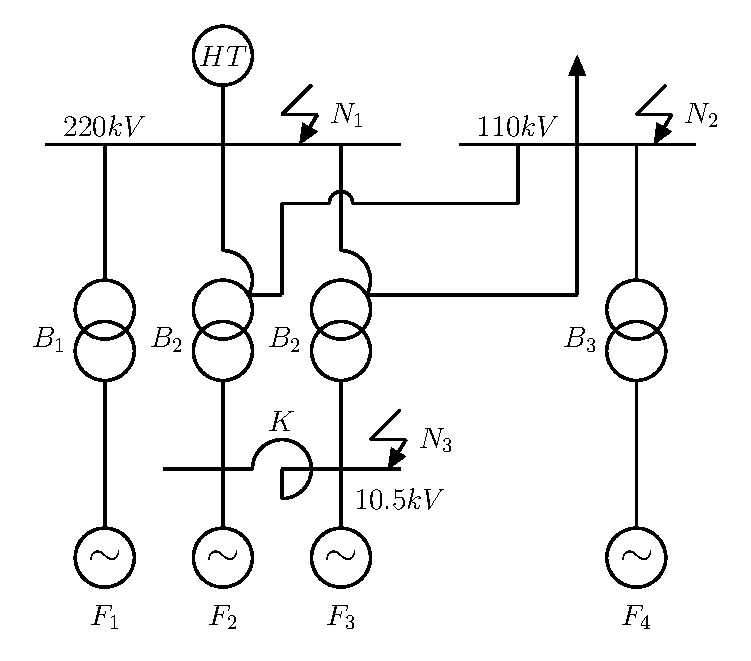
\includegraphics[scale=1]{figure-baitap-nganmach-1.pdf}
\end{center}
\caption{Sơ đồ nguyên lý}\label{Fig:baitap-ngan-mach-1}
\end{figure}

%%---------------------------------------------
%% Dữ liệu ban đầu
%% Đơn vị KVA, KV
%Xây dựng các hàm tính toán cho một số giá trị
\begin{sagesilent}
def dongcoban(Scoban,Ucoban,error):
  return round((Scoban/(sqrt(3)*Ucoban)),error)
  
def dienkhanghethong1(xdinhmuc,Scoban,Shethong,error):
  return round(xdinhmuc*Scoban/Shethong,error)
  
def dienkhangduongday(xdonvi,chieudai,Scoban,Ucoban,error):
  return round(xdonvi*chieudai*Scoban/Ucoban^2,error)
  
def dienkhangmaybienap(dienap_nganmach, Scoban, Sdinhmuc,error):
  return round(dienap_nganmach/100*Scoban/Sdinhmuc,error)
  
def dienap_nganmach_bienaptungau(hesotungau, Ucaotrung, Ucaoha, Utrungha, error):
  #Tính toán điện áp ngắn mạch ở các cuộn dây: cao, trung, hạ
  Unganmach_cao = round(0.5*(Ucaotrung + Ucaoha/hesotungau - Utrungha/hesotungau),error)
  Unganmach_trung = round(0.5*(Ucaotrung + Utrungha/hesotungau - Ucaoha/hesotungau),error)
  Unganmach_ha = round(0.5*(Ucaoha/hesotungau + Utrungha/hesotungau - Ucaotrung),error)
  
  Unganmach = [Unganmach_cao, Unganmach_trung, Unganmach_ha]
  
  for i in range(len(Unganmach)): #So sánh điện áp ngắn mạch với 0
  	if Unganmach[i] < 0:
  	  Unganmach[i] = 0
  return Unganmach
  
def dienkhangcuonkhang(xkhang, Icoban, Idinhmuckhang,error):	#Tính giá trị điện kháng cuộn kháng
  return round(xkhang/100*Icoban/Idinhmuckhang,error)
  
def dienkhangmayphat(xsieuquado, Scoban, Sdinhmuc,error): #Điện kháng máy phát
  return round(xsieuquado/100*Scoban/Sdinhmuc,error)
  
def dongnganmach_coban(dienkhangtuongduong,error):
  dongcoban = []
  for i in dienkhangtuongduong:
    dongcoban.append(round(i^-1, error))
  return dongcoban
  
def dongnganmachdonvi(dong_nganmach_coban, dongcoban, error):
  dongdonvi = []
  for i in range(len(dongcoban)):
    dongdonvi.append(round(dong_nganmach_coban[i]*dongcoban[i],error))
  return dongdonvi

\end{sagesilent}

\begin{sagesilent}
n = 4; # Làm tròn 4 chữ số thập phân

### Phần tử hệ thống
S_HT = 5000; U_HT = 220; xdm = round(0.3,1);

### Phần tử máy phát
S_MP = 125; U_MP = round(10.5,1); xd = round(0.192,3);

### Phần tử máy biến áp
S_BA1 = 125; U_N1 = 11;
S_BA2 = 125; U_NCH = 31; U_NCT = 11; U_NTH = 19; k = round(0.5,1);
S_BA3 = 125; U_N3 = round(10.5,1);

### Phần tử đường dây
U_DD = 220; l = 100; x0 = round(0.4,1);

### Phần tử kháng điện
xk = 10; I_dm = 3000; U_dm = round(10.5,1);

#### Áp dụng công thức giải:

Scb = 1000;	#Giá trị công suất cơ bản
Ucb = [230, 115,round(10.5,1)];	#Giải trị điện áp cơ bản tại thanh cái

#Tính giá trị dòng cơ bản
Icb = [];
for i in Ucb:
  Icb.append(dongcoban(Scb,i,n))
  
# Tính các giá trị điện kháng
X1b1 = dienkhanghethong1(xdm,Scb,S_HT,n);	#Điện kháng của hệ thống

X2b1 = dienkhangduongday(x0,l,Scb,Ucb[0],n);	#Điện kháng đường dây

X3b1 = dienkhangmaybienap(U_N1,Scb,S_BA1,n); #Điện kháng máy biến áp

X4b1 = dienkhangmaybienap(U_N3,Scb,S_BA3,n); #Điện kháng máy biến áp

UN_BA2 = dienap_nganmach_bienaptungau(k, U_NCT, U_NCH, U_NTH,n); # Điện áp ngắn mạch các cuộn của biến áp tự ngẫu
X_BA2 = []
for i in UN_BA2:		# Điện kháng các cuộn máy biến áp tự ngẫu
  X_BA2.append(dienkhangmaybienap(i,Scb,S_BA2,n))
  
X8b1 = dienkhangcuonkhang(xk, Icb[2], I_dm/1000,n); #Điện kháng cuộn kháng

X9b1 = dienkhangmayphat(xd*100, Scb, S_MP,n); #Điện kháng máy phát

X5b1 = X_BA2[0];	 #Điện kháng cuộn cao
X7b1 = X_BA2[2]; #Điện kháng cuộn hạ
#Tính các giá trị điện kháng tổng hợp trên sơ đồ
X10b1 = round(X3b1+X9b1,n)
X11b1 = round(X7b1+X9b1,n)
X12b1 = round(X4b1+X9b1,n)
X13b1 = round(X5b1/2,n)
X14b1 = round(X2b1/2,n)
X15b1 = round(X1b1+X14b1,n)
X16b1 = round((1/X11b1 + 1/X11b1 + 1/X12b1)^-1,n)
X17b1 = round(X16b1+X13b1,n)
XSigmaN1b1 = round((1/X10b1 + 1/X15b1 + 1/X17b1)^-1,n)

#Điểm ngắn mạch N2
X18b1 = round((1/X10b1 + 1/X15b1)^-1,n)
X19b1 = round(X18b1 + X13b1,n)
XSigmaN2b1 = round((1/X16b1 + 1/X19b1)^-1,n)

#Điểm ngắn mạch N3
X20b1 = round(X7b1*X8b1/(2*X7b1+X8b1),n)
X21b1 = round(X7b1*X8b1/(2*X7b1+X8b1),n)
X22b1 = round(X7b1*X7b1/(2*X7b1+X8b1),n)
X23b1 = round(X9b1 + X20b1,n)
X24b1 = round((1/X12b1 + 1/X19b1)^-1,n)
X25b1 = round(X22b1 + X24b1,n)
X26b1 = round((1/X23b1 + 1/X25b1)^-1,n)
X27b1 = round(X21b1 + X26b1,n)
XSigmaN3b1 = round((1/X9b1 + 1/X27b1)^-1,n)

dienkhangtonghopb1 = [XSigmaN1b1, XSigmaN2b1, XSigmaN3b1]

dongcobanb1 = dongnganmach_coban(dienkhangtonghopb1,n)

dongdonvib1 = dongnganmachdonvi(dongcobanb1, Icb, n)

#Hệ số xung kích: 
kxkb1 = round(1.8,1)

Ikxkb1 = []
for i in dongdonvib1:
  Ikxkb1.append(round(kxkb1*i*sqrt(2),n))
\end{sagesilent} 

\item \textit{Hệ thống:} $\vidss{S}{$\Sigma$} = \sage{S_HT} \unit{MVA}; U_{HT} = \sage{U_HT} \unit{kV}; \viss{x}^\ast = \sage{xdm}$.
\item \textit{Máy phát điện $F$}: nhiệt điện $$F_1 = F_2 = F_3 = F_4; \viss{S} = \sage{S_MP} \unit{MVA}; \viss{U} = \sage{U_MP} \unit{kV}; x_d^{\prime \prime} = \sage{xd}$$
\item \textit{Máy biến áp:}
\begin{equation*}
\begin{split}
B_1 &: \viss{S} = \sage{S_BA1}\unit{MVA}; U_N\% =  \sage{U_N1}\\
B_2 &: \viss{S} =  \sage{S_BA2} \unit{MVA}; U_N\%_{CH} = \sage{U_NCH}; U_N\%_{CT} = \sage{U_NCT}; U_N\%_{TH} = \sage{U_NTH}\\
B_3 &: \viss{S} =  \sage{S_BA3} \unit{MVA}; U_N\% = \sage{U_N3}
\end{split}
\end{equation*}
\item  \textit{Đường dây kép:} $\sage{U_DD}\unit{kV};l = \sage{l} \unit{km}$.
\item \textit{Kháng điện:} $x_k \%= \sage{xk}\%; \viss{I}=\sage{I_dm}\unit{A}; \viss{U} = \sage{U_dm} \unit{kV}$.
\end{itemize}

\subparagraph{Yêu cầu} Tính ngắn mạch tại các điểm $N_1,N_2,N3$.

\subparagraph{Bài giải}
\begin{itemize}
	\item \textit{Bước 1:} Vẽ sơ đồ mô hình hóa của hệ thống: hình \ref{Fig:sodo-mohinhhoa-bt1}.
		\begin{figure}[!h]
			\begin{center}
				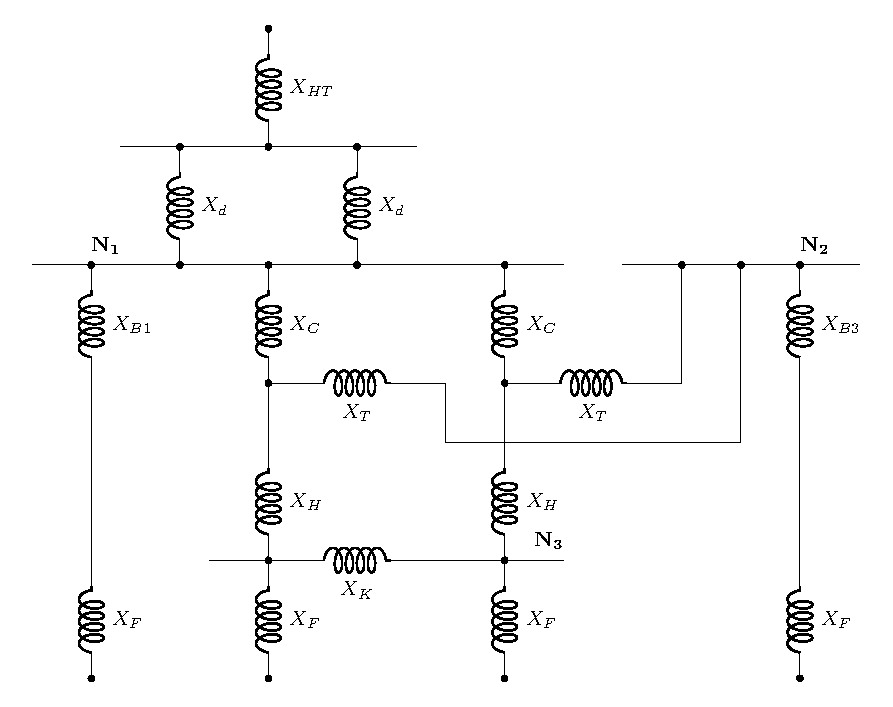
\includegraphics[scale=1]{figure-baitap-nganmach-1-1.pdf} 
			\end{center}
			\caption{Sơ đồ mô hình hóa} \label{Fig:sodo-mohinhhoa-bt1}
		\end{figure}

	\item \textit{Bước 2:} Chọn $S_{cb}$ và $U_{cb}$ để tính $I_{cb}$.	
		\begin{itemize}
			\item Chọn $S_{cb} = \sage{Scb} \unit{MVA}$ và $U_{cb} = \sage{Ucb} \unit{kV}$.
			
			\item Tính giá trị dòng điện cơ bản:
				\begin{equation*}
					\begin{split}
						I_{cb\left({220kV}\right)} & = \dfrac{S_{cb}}{\sqrt{3} \times U_{cb_{1}}} = \dfrac{\sage{Scb}}{\sqrt{3} \times \sage{Ucb[0]}} = \sage{Icb[0]} \unit{kA}\\
						I_{cb\left({110kV}\right)} & = \dfrac{S_{cb}}{\sqrt{3} \times U_{cb_{2}}} = \dfrac{\sage{Scb}}{\sqrt{3} \times \sage{Ucb[1]}} = \sage{Icb[1]} \unit{kA}\\
						I_{cb\left({10.5kV}\right)} & = \dfrac{S_{cb}}{\sqrt{3} \times U_{cb_{3}}} = \dfrac{\sage{Scb}}{\sqrt{3} \times \sage{Ucb[2]}} = \sage{Icb[2]} \unit{kA}
					\end{split}
				\end{equation*}
		\end{itemize}

	\newpage
	\item \textit{Bước 3}: Tính giá trị điện kháng của các phần tử trong hệ thống.
		\begin{itemize}
		
			\item Hệ thống: $X_1 = X_{HT} = \viss{x}^\ast \times \dfrac{S_{cb}}{S_{\Sigma HT}}=\sage{xdm}\times \dfrac{\sage{Scb}}{\sage{S_HT}} = \sage{X1b1}$
			
			\item Đường dây kép: $X_2 = X_d = x_0 \times l \times \dfrac{S_{cb}}{U_{cb_{1}}^2} = \sage{x0} \times \sage{l} \times \dfrac{\sage{Scb}}{\sage{Ucb[0]}^2} = \sage{X2b1}$
			
			\item Máy biến áp $B_1$: $X_3 = X_{B1} = \dfrac{U_N\%}{100} \times \dfrac{S_{cb}}{\viss{S}} = \dfrac{\sage{U_N1}}{100}\times \dfrac{\sage{Scb}}{\sage{S_BA1}}=\sage{X3b1}$
			
			\item Máy biến áp $B_3$: $X_4 = X_{B3} = \dfrac{U_N\%}{100} \times \dfrac{S_{cb}}{\viss{S}} = \dfrac{\sage{U_N3}}{100}\times \dfrac{\sage{Scb}}{\sage{S_BA3}}=\sage{X4b1}$

			\item Máy biến áp tự ngẫu $B2$:
				\begin{list}{+}{}
					\item Tính điện áp ngắn mạch trên các cuộn:
						\begin{align*}						
						U_N\%_C & = \dfrac{1}{2} \times \pfm{ U_N\%_{CT} + \dfrac{U_N\%_{CH}}{\alpha} - \dfrac{U_N\%_{TH}}{\alpha} } = \dfrac{1}{2} \times \pfm{ \sage{U_NCT} + \dfrac{\sage{U_NCH}}{\sage{k}} - \dfrac{\sage{U_NTH}}{\sage{k}} } = \sage{UN_BA2[0]}\\
						U_N\%_T & = \dfrac{1}{2} \times \pfm{ U_N\%_{CT} + \dfrac{U_N\%_{TH}}{\alpha} - \dfrac{U_N\%_{CH}}{\alpha} } = \dfrac{1}{2} \times \pfm { \sage{U_NCT} + \dfrac{\sage{U_NTH}}{\sage{k}} - \dfrac{\sage{U_NCH}}{\sage{k}} } = \sage{UN_BA2[1]}\\		
						U_N\%_H & = \dfrac{1}{2} \times \pfm{ \dfrac{U_N\%_{CH}}{\alpha} + \dfrac{U_N\%_{TH}}{\alpha} - U_N\%_{CT} } = \dfrac{1}{2} \times \pfm{ \dfrac{\sage{U_NCH}}{\sage{k}} + \dfrac{\sage{U_NTH}}{\sage{k}} - \sage{U_NCT} } = \sage{UN_BA2[2]}
						\end{align*}
					
					\item Điện kháng cơ bản trên các cuộn:
						\begin{equation*}
							\begin{split}
								X_5 = X_C & = \dfrac{U_N\%_C}{100} \times \dfrac{S_{cb}}{\viss{S}} = \dfrac{\sage{UN_BA2[0]}}{100}\times \dfrac{\sage{Scb}}{\sage{S_BA2}} = \sage{X_BA2[0]}\\
								X_6 = X_T & = \dfrac{U_N\%_T}{100} \times \dfrac{S_{cb}}{\viss{S}} = \dfrac{\sage{UN_BA2[1]}}{100}\times \dfrac{\sage{Scb}}{\sage{S_BA2}} = \sage{X_BA2[1]}\\
								X_7 = X_H & = \dfrac{U_N\%_H}{100} \times \dfrac{S_{cb}}{\viss{S}} = \dfrac{\sage{UN_BA2[2]}}{100}\times \dfrac{\sage{Scb}}{\sage{S_BA2}} = \sage{X_BA2[2]}
							\end{split}
						\end{equation*}
				\end{list}

			\item Kháng điện: $ X_8 = X_K = \dfrac{x_K\%}{100} \times \dfrac{I_{cb_{2}}}{\viss{I}} = \dfrac{\sage{xk}}{100}\times \frac{\sage{Icb[2]}}{\sage{I_dm}\times 10^{-3}} = \sage{X8b1}$
			
			\item Máy phát: $ X_9 = X_F = \frac{x_{d}^{\prime\prime}\%}{100} \times \frac{S_{cb}}{\viss{S}} = \frac{\sage{xd}\times 100}{100}\times \frac{\sage{Scb}}{\sage{S_MP}} = \sage{X9b1}$
		\end{itemize}
		
	\item \textit{Bước 4}: Biến đổi về sơ đồ đẳng trị cho từng điểm ngắn mạch.
		\begin{itemize}
			\item \textbf{\textit{Điểm ngắn mạch N1}}
				\begin{itemize}
					\item Do $X_T = 0 $ và $X_K$ không ảnh hưởng đến điểm ngắn mạch $N_1$, nên bỏ qua, được sơ đồ hình \ref{Fig:sodo-tuongduong-bt1-N1-1}. Ta có:
					\begin{figure}[!h]
						\begin{center}
							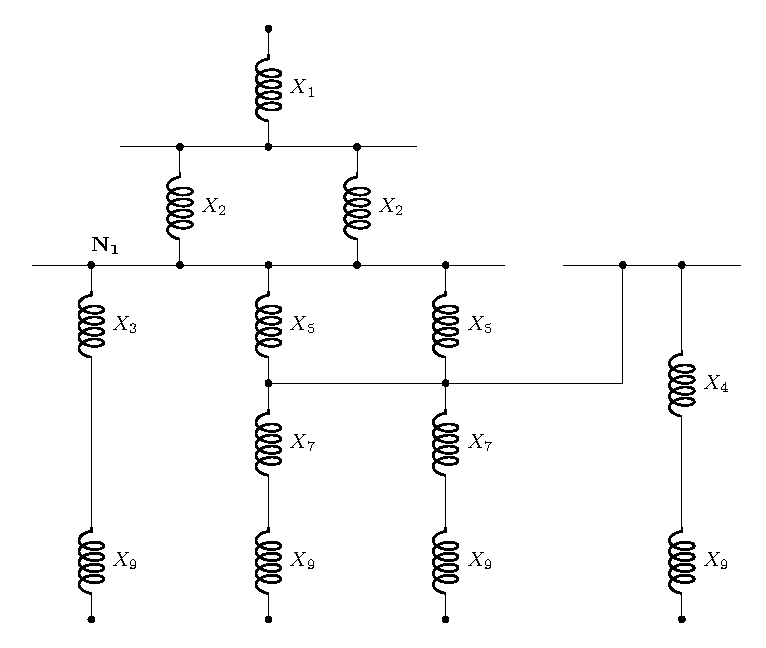
\includegraphics[scale=1]{figure-baitap-nganmach-1-N1-1.pdf} 
						\end{center}
						\caption{Sơ đồ tương đương 1 cho điểm ngắn mạch $N_1$} \label{Fig:sodo-tuongduong-bt1-N1-1}
						
					\end{figure}

					\begin{list}{+}{}
						\item $X_{10} = X_3 \textrm{ nt } X_9 $: $X_{10} = X_3 + X_9 = \sage{X3b1} + \sage{X9b1} = \sage{X10b1}$

						\item $X_{11} = X_7 \textrm{ nt } X_9 $: $X_{11} = X_7 + X_9 = \sage{X7b1} + \sage{X9b1} = \sage{X11b1}$

						\item $X_{12} = X_4 \textrm{ nt } X_9 $: $X_{12} = X_4 + X_9 = \sage{X4b1} + \sage{X9b1} = \sage{X12b1}$
						
						\item $X_{13} = X_5 \textrm{ ss } X_5 $: $X_{13} = \dfrac{X_5}{2} = \dfrac{\sage{X5b1}}{2} = \sage{X13b1}$
						
						\item $X_{14} = X_2 \textrm{ ss } X_2 $: $X_{14} = \dfrac{X_2}{2} = \dfrac{\sage{X2b1}}{2} = \sage{X14b1}$

						\item $X_{15} = X_1 \textrm{ nt } X_{14} $: $X_{15} = X_1 + X_{14} = \sage{X1b1} + \sage{X14b1} = \sage{X15b1}$
						
					\end{list}
				
				\newpage
				\item Sơ đồ tương đương 2 cho điểm $N_1$: hình \ref{Fig:sodo-tuongduong-bt1-N1-2}. Ta có
					\begin{figure}[!h]
						\begin{center}
							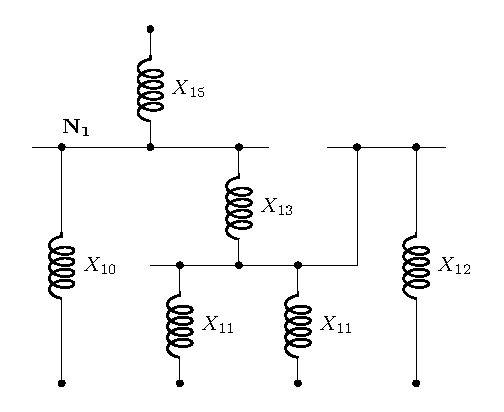
\includegraphics[scale=1]{figure-baitap-nganmach-1-N1-2.pdf} 
						\end{center}
					\caption{Sơ đồ tương đương 2 cho điểm ngắn mạch $N_1$} \label{Fig:sodo-tuongduong-bt1-N1-2}
					\end{figure}

					\begin{list}{+}{}
						\item $X_{16} = X_{11} \textrm{ ss } X_{11} \textrm{ ss } X_{12}:$ $$ \dfrac{1}{X_{16}} = \dfrac{1}{X_{11}} + \dfrac{1}{X_{11}} + \dfrac{1}{X_{12}} = \dfrac{1}{\sage{X11b1}} + \dfrac{1}{\sage{X11b1}} + \dfrac{1}{\sage{X12b1}} \Longrightarrow X_{16} = \sage{X16b1}$$
						
						\item $X_{17} = X_{16} \textrm{ nt } X_{13}: X_{17} = X_{13} + X_{16} = \sage{X13b1} + \sage{X16b1} = \sage{X17b1}$
						
					\end{list}

				\newpage
				\item Sơ đồ tương đương 3 cho điểm $N_1$: hình \ref{Fig:sodo-tuongduong-bt1-N1-3}.
					\begin{figure}[!h]
						\vspace{-.5cm}
						\begin{center}
							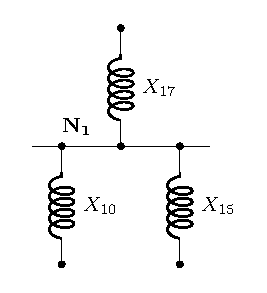
\includegraphics[scale=1]{figure-baitap-nganmach-1-N1-3.pdf} 
							\vspace{-.5cm}
						\end{center}
						\caption{Sơ đồ tương đương 3 cho điểm ngắn mạch $N_1$} \label{Fig:sodo-tuongduong-bt1-N1-3}
					\end{figure}

					Ta có: $X_{\Sigma N1} = X_{10} \textrm{ ss } X_{15} \textrm{ ss } X_{17}:$ $$ \dfrac{1}{X_{\Sigma N1}} = \dfrac{1}{X_{10}} + \dfrac{1}{X_{15}} + \dfrac{1}{X_{17}} = \dfrac{1}{\sage{X10b1}} + \dfrac{1}{\sage{X15b1}} + \dfrac{1}{\sage{X17b1}} \Longrightarrow X_{\Sigma N1} = \sage{XSigmaN1b1}$$
				\end{itemize}
			
			\item \textbf{\textit{Điểm ngắn mạch N2}}
				\begin{itemize}
					\item Do $X_T = 0 $ và $X_K$ không ảnh hưởng đến điểm ngắn mạch $N_2$, nên bỏ qua, được sơ đồ hình \ref{Fig:sodo-tuongduong-bt1-N2-1}. Ta có:
					\begin{figure}[!h]
						\vspace{-.5cm}
						\begin{center}
							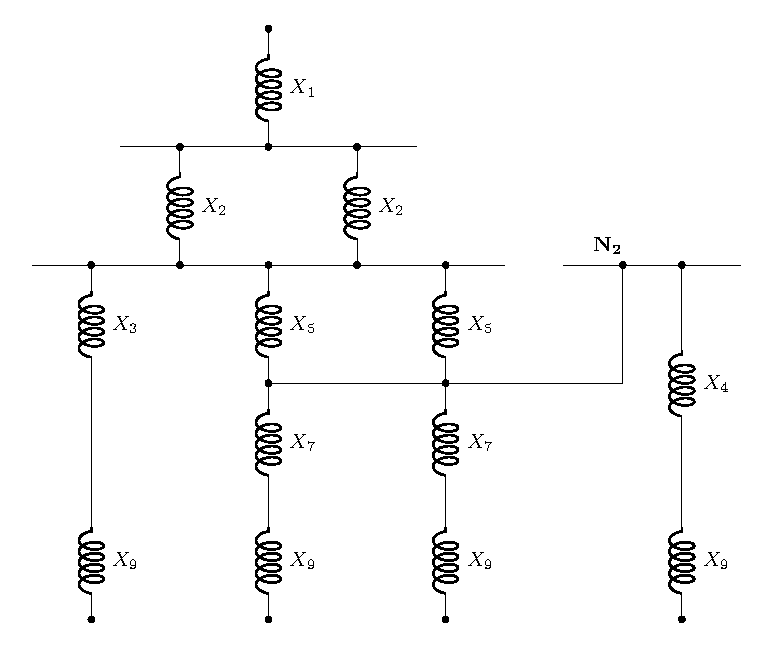
\includegraphics[scale=1]{figure-baitap-nganmach-1-N2-1.pdf} 
							\vspace{-.5cm}
						\end{center}
						\caption{Sơ đồ tương đương 1 cho điểm ngắn mạch $N_2$} \label{Fig:sodo-tuongduong-bt1-N2-1}
					\end{figure}

					\begin{list}{+}{}
						\item $X_{10} = X_3 \textrm{ nt } X_9 $: $X_{10} = X_3 + X_9 = \sage{X3b1} + \sage{X9b1} = \sage{X10b1}$

						\item $X_{11} = X_7 \textrm{ nt } X_9 $: $X_{11} = X_7 + X_9 = \sage{X7b1} + \sage{X9b1} = \sage{X11b1}$

						\item $X_{12} = X_4 \textrm{ nt } X_9 $: $X_{12} = X_4 + X_9 = \sage{X4b1} + \sage{X9b1} = \sage{X12b1}$
						
						\item $X_{13} = X_5 \textrm{ ss } X_5 $: $X_{13} =  \dfrac{X_5}{2} = \dfrac{\sage{X5b1}}{2} = \sage{X13b1}$
						
						\item $X_{14} = X_2 \textrm{ ss } X_2 $: $X_{14} = \dfrac{X_2}{2} = \dfrac{\sage{X2b1}}{2} = \sage{X14b1}$

						\item $X_{15} = X_1 \textrm{ nt } X_{14} $: $X_{15} = X_1 + X_{14} = \sage{X1b1} + \sage{X14b1} = \sage{X15b1}$
					\end{list}
				
					\item Sơ đồ tương đương 2 cho điểm $N_2$: hình \ref{Fig:sodo-tuongduong-bt1-N2-2}. Ta có:
					\begin{figure}[!h]
						\begin{center}
							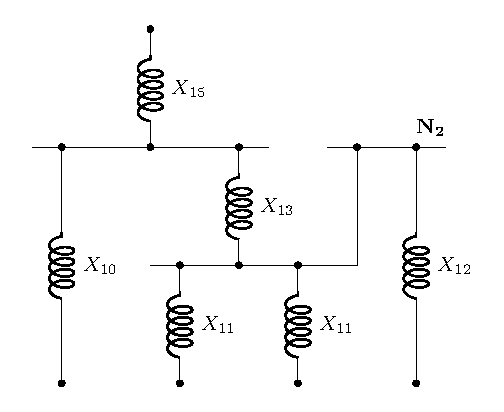
\includegraphics[scale=1]{figure-baitap-nganmach-1-N2-2.pdf} 
						\end{center}
					\caption{Sơ đồ tương đương 2 cho điểm ngắn mạch $N_2$} \label{Fig:sodo-tuongduong-bt1-N2-2}
					\end{figure}

					\begin{list}{+}{}
						\item $X_{16} = X_{11} \textrm{ ss } X_{11} \textrm{ ss } X_{12}:$ $$ \dfrac{1}{X_{16}} = \dfrac{1}{X_{11}} + \dfrac{1}{X_{11}} + \dfrac{1}{X_{12}} = \dfrac{1}{\sage{X11b1}} + \dfrac{1}{\sage{X11b1}} + \dfrac{1}{\sage{X12b1}} \Longrightarrow X_{16} = \sage{X16b1}$$

						\item $X_{18} = X_{10} \textrm{ ss } X_{15}:$ $$\dfrac{1}{X_{18}} = \dfrac{1}{X_{10}} + \dfrac{1}{X_{15}} = \dfrac{1}{\sage{X10b1}} + \dfrac{1}{\sage{X15b1}} \Longrightarrow X_{18} = \sage{X18b1}$$
					\end{list}
					
					\item Sơ đồ tương đương 3 cho điểm $N_2$: hình \ref{Fig:sodo-tuongduong-bt1-N2-3}. Ta có:
					\begin{figure}[!h]
						\begin{center}
							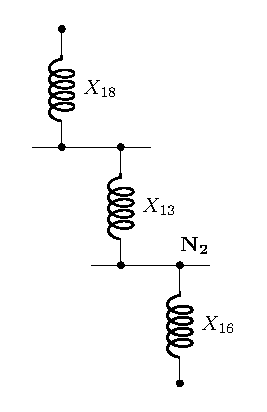
\includegraphics[scale=1]{figure-baitap-nganmach-1-N2-3.pdf} 
						\end{center}
					\caption{Sơ đồ tương đương 3 cho điểm ngắn mạch $N_2$} \label{Fig:sodo-tuongduong-bt1-N2-3}
					\end{figure}
					
					\begin{list}{+}{}
						\item $X_{19} = X_{18} \textrm{ nt } X_{13}: X_{19} = X_{18} + X_{13} = \sage{X18b1} + \sage{X13b1} = \sage{X19b1}$
						
						\item $X_{\Sigma N2} = X_{16} \textrm{ ss } X_{19}:$ $$\dfrac{1}{X_{\Sigma N2}} = \dfrac{1}{X_{16}} +  \dfrac{1}{X_{19}} +  = \dfrac{1}{\sage{X16b1}} + \dfrac{1}{\sage{X19b1}} \Longrightarrow  X_{\Sigma N2} = \sage{XSigmaN2b1} $$

					\end{list}										
				\end{itemize}
			
			\newpage
			\item \textbf{\textit{Điểm ngắn mạch N3}}
				\begin{itemize}
					\item Do $X_T = 0 $ nên bỏ qua, được sơ đồ hình \ref{Fig:sodo-tuongduong-bt1-N3-1}. Ta có:
					\begin{figure}[!h]
						\begin{center}
							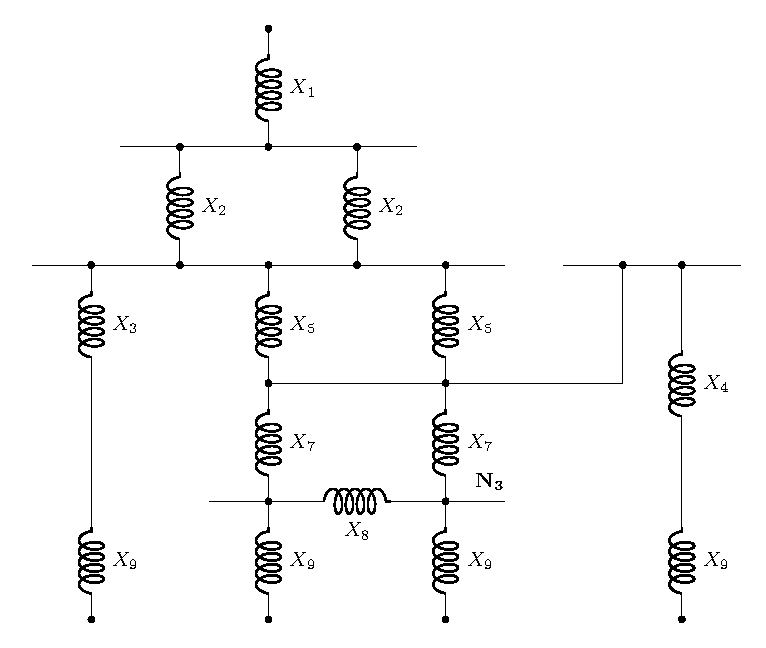
\includegraphics[scale=1]{figure-baitap-nganmach-1-N3-1.pdf} 
						\end{center}
					\caption{Sơ đồ tương đương 1 cho điểm ngắn mạch $N_3$} \label{Fig:sodo-tuongduong-bt1-N3-1}
					\end{figure}
					
					\begin{list}{+}{}
						\item $X_{10} = X_3 \textrm{ nt } X_9 $: $X_{10} = X_3 + X_9 = \sage{X3b1} + \sage{X9b1} = \sage{X10b1}$			

						\item $X_{12} = X_4 \textrm{ nt } X_9 $: $X_{12} = X_4 + X_9 = \sage{X4b1} + \sage{X9b1} = \sage{X12b1}$
						
						\item $X_{13} = X_5 \textrm{ ss } X_5 $: $X_{13} =  \dfrac{X_5}{2} = \dfrac{\sage{X5b1}}{2} = \sage{X13b1}$
						
						\item $X_{14} = X_2 \textrm{ ss } X_2 $: $X_{14} = \dfrac{X_2}{2} = \dfrac{\sage{X2b1}}{2} = \sage{X14b1}$

						\item $X_{15} = X_1 \textrm{ nt } X_{14} $: $X_{15} = X_1 + X_{14} = \sage{X1b1} + \sage{X14b1} = \sage{X15b1}$
						
						\item Biến đổi $\Delta - Y$ cho $X_7, X_7, X_8$:
							\begin{align*}
								X_{20} = \dfrac{X_7 \times X_8}{X_7 + X_7 + X_8} & = \dfrac{\sage{X7b1} \times \sage{X8b1}}{\sage{X7b1} + \sage{X7b1} + \sage{X8b1}} = \sage{X20b1} \\
								X_{21} = \dfrac{X_7 \times X_8}{X_7 + X_7 + X_8} & = \dfrac{\sage{X7b1} \times \sage{X8b1}}{\sage{X7b1} + \sage{X7b1} + \sage{X8b1}} = \sage{X21b1} \\
								X_{22} = \dfrac{X_7 \times X_7}{X_7 + X_7 + X_8} & = \dfrac{\sage{X7b1} \times \sage{X7b1}}{\sage{X7b1} + \sage{X7b1} + \sage{X8b1}} = \sage{X22b1}
							\end{align*}
					\end{list}
					\newpage
					\item Sơ đồ tương đương 2 cho điểm $N_3$: hình \ref{Fig:sodo-tuongduong-bt1-N3-2}. Ta có:
					\begin{figure}[!h]
						\begin{center}
							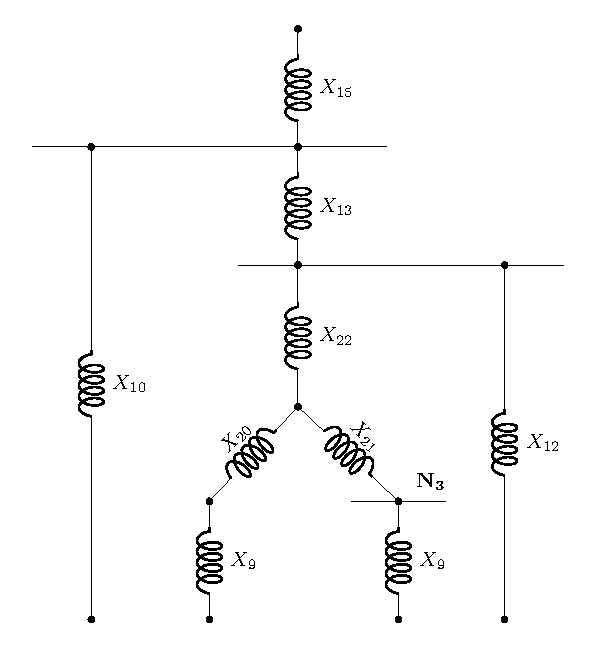
\includegraphics[scale=1]{figure-baitap-nganmach-1-N3-2.pdf} 
						\end{center}
					\caption{Sơ đồ tương đương 2 cho điểm ngắn mạch $N_3$} \label{Fig:sodo-tuongduong-bt1-N3-2}
					\end{figure}
					
					\begin{list}{+}{}
						\item $X_{18} = X_{10} \textrm{ ss } X_{15}:$ $$\dfrac{1}{X_{18}} = \dfrac{1}{X_{10}} + \dfrac{1}{X_{15}} = \dfrac{1}{\sage{X10b1}} + \dfrac{1}{\sage{X15b1}} \Longrightarrow X_{18} = \sage{X18b1}$$
						
						\item $X_{19} = X_{18} \textrm{ nt } X_{13}: X_{19} = X_{18} + X_{13} = \sage{X18b1} + \sage{X13b1} = \sage{X19b1}$
						\item $X_{23} = X_{9} \textrm{ nt } X_{20}: X_{23} = X_{9} + X_{20} = \sage{X9b1} + \sage{X20b1} = \sage{X23b1}$
					\end{list}
					
					\item Sơ đồ tương đương 3 cho điểm $N_3$: hình \ref{Fig:sodo-tuongduong-bt1-N3-3}. Ta có:
					\begin{figure}[!h]
						\vspace{-.5cm}
						\begin{center}
							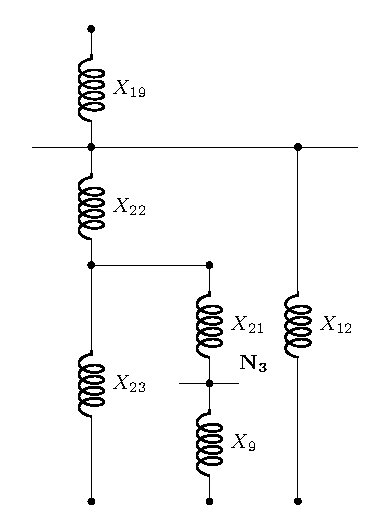
\includegraphics[scale=1]{figure-baitap-nganmach-1-N3-3.pdf} 
							\vspace{-.5cm}
						\end{center}
					\caption{Sơ đồ tương đương 3 cho điểm ngắn mạch $N_3$} \label{Fig:sodo-tuongduong-bt1-N3-3}
					\vspace{-.5cm}
					\end{figure}
					
					\begin{list}{+}{}
						\item $X_{24} = X_{12} \textrm{ ss } X_{19}:$ $$\dfrac{1}{X_{24}} = \dfrac{1}{X_{12}} + \dfrac{1}{X_{19}} = \dfrac{1}{\sage{X12b1}} + \dfrac{1}{\sage{X19b1}} \Longrightarrow X_{24} = \sage{X24b1}$$
						
						\item $X_{25} = X_{22} \textrm{ nt } X_{24}: X_{25} = X_{22} + X_{24} = \sage{X22b1} + \sage{X24b1} = \sage{X25b1}$
						
						\item $X_{26} = X_{23} \textrm{ ss } X_{25}:$ $$\dfrac{1}{X_{26}} = \dfrac{1}{X_{23}} + \dfrac{1}{X_{25}} = \dfrac{1}{\sage{X23b1}} + \dfrac{1}{\sage{X25b1}} \Longrightarrow X_{26} = \sage{X26b1}$$
						
						\item $X_{27} = X_{21} \textrm{ nt } X_{26}: X_{27} = X_{21} + X_{26} = \sage{X21b1} + \sage{X26b1} = \sage{X27b1}$
						
						\item $X_{\Sigma N3} = X_{9} \textrm{ ss } X_{27}:$ $$\dfrac{1}{X_{\Sigma N3}} = \dfrac{1}{X_{9}} +  \dfrac{1}{X_{27}} +  = \dfrac{1}{\sage{X9b1}} + \dfrac{1}{\sage{X27b1}} \Longrightarrow  X_{\Sigma N3} = \sage{XSigmaN3b1} $$
					\end{list}
			\end{itemize}
			\item \textit{Bước 5:} Tính dòng điện ngắn mạch tại các điểm $N1, N2, N3$.
				\begin{equation*}
					\begin{split}
						I_{N1}^\ast & = \dfrac{1}{X_{\Sigma N1}} = \dfrac{1}{\sage{dienkhangtonghopb1[0]}} = \sage{dongcobanb1[0]} \Longrightarrow I_{N1} = I_{N1}^\ast \times I_{cb N1} = \sage{dongcobanb1[0]} \times \sage{Icb[0]} = \sage{dongdonvib1[0]}\unit{kA} \\			
						I_{N2}^\ast & = \dfrac{1}{X_{\Sigma N2}} = \dfrac{1}{\sage{dienkhangtonghopb1[1]}} = \sage{dongcobanb1[1]} \Longrightarrow I_{N2} = I_{N2}^\ast \times I_{cb N2} = \sage{dongcobanb1[1]} \times \sage{Icb[1]} = \sage{dongdonvib1[1]}\unit{kA}	\\
						I_{N3}^\ast & = \dfrac{1}{X_{\Sigma N3}} = \dfrac{1}{\sage{dienkhangtonghopb1[2]}} = \sage{dongcobanb1[2]} \Longrightarrow I_{N3} = I_{N3}^\ast \times I_{cb N3} = \sage{dongcobanb1[2]} \times \sage{Icb[2]} = \sage{dongdonvib1[2]}\unit{kA}						
					\end{split}
			\end{equation*}

			\item \textit{Bước 6}: Chọn hệ số xung kích $k_{xk}$.
			
			Với công suất biểu kiến của máy biến áp, ta có: $k_{xk} = \sage{kxkb1}$
			
			\item \textit{Bước 7}: Tính dòng điện ngắn mạch xung kích.
				\begin{align*}					
						I_{xk N1} & = \sqrt{2}\times I_{N1}\times k_{xk} = \sqrt{2}\times \sage{dongdonvib1[0]} \times \sage{kxkb1} = \sage{Ikxkb1[0]} \unit{kA}\\
						I_{xk N2} & = \sqrt{2}\times I_{N2}\times k_{xk} = \sqrt{2}\times \sage{dongdonvib1[1]} \times \sage{kxkb1} = \sage{Ikxkb1[1]} \unit{kA}\\
						I_{xk N3} & = \sqrt{2}\times I_{N3}\times k_{xk} = \sqrt{2}\times \sage{dongdonvib1[2]} \times \sage{kxkb1} = \sage{Ikxkb1[2]} \unit{kA}
				\end{align*}	
				
				\item \textit{Bước 8}: Tổng hợp kết quả tính toán vào bảng \ref{Tab:tonghop-ketqua-b1}.
					\begin{table}[!h]
					\begin{normalsize}
						\begin{center}
							\begin{tabular}{|c|p{1.cm}|p{1cm}|p{1.5cm}|p{3cm}|c|c|p{1.3cm}|p{1.5cm}|}\hline
								STT & Điểm ngắn mạch & $\viss{U}$ $\pfm{kV}$ & Thành phần tham gia & Mục đích tính toán & $X_\Sigma$ & $I_{cb}^\ast$ & $I_N$ $\pfm{kA}$ & $I_{xk}$ $\pfm{kA}$\\ \hline
							$1$ & $N1$ & $220$ & Tất cả & Chọn các khí cụ điện cấp $220kV$ & $\sage{dienkhangtonghopb1[0]}$  & $\sage{dongcobanb1[0]}$ & $\sage{dongdonvib1[0]}$ & $\sage{Ikxkb1[0]}$\\ \hline
							$2$ & $N2$ & $110$ & Tất cả & Chọn các khí cụ điện cấp $110kV$ & $\sage{dienkhangtonghopb1[1]}$  & $\sage{dongcobanb1[1]}$ & $\sage{dongdonvib1[1]}$ & $\sage{Ikxkb1[1]}$\\ \hline
							
							$3$ & $N3$ & $10.5$ & Tất cả & Chọn các khí cụ điện cấp $10.5kV$ & $\sage{dienkhangtonghopb1[2]}$  & $\sage{dongcobanb1[2]}$ & $\sage{dongdonvib1[2]}$ & $\sage{Ikxkb1[2]}$\\ \hline
							\end{tabular}
						\end{center}		
				\end{normalsize}
				\caption{Kết quả tính toán các điểm ngắn mạch trong bài 1} \label{Tab:tonghop-ketqua-b1}
				\end{table}
		\end{itemize}
\end{itemize}
\end{document}